\documentclass{notices}

\usepackage[usenames,dvipsnames,svgnames,table]{xcolor}
%\usepackage[colorlinks=true, pdfstartview=FitV, linkcolor=blue, citecolor=blue, urlcolor=darkblue]%{hyperref}

%\usepackage{addfont}
%\addfont{OT1}{rsfs10}{\rsfs}

\usepackage{geometry}                % See geometry.pdf to learn the layout options. There are lots.
\geometry{letterpaper}                   % ... or a4paper or a5paper or ...
%\geometry{landscape}                % Activate for for rotated page geometry
%\usepackage[parfill]{parskip}    % Activate to begin paragraphs with an empty line rather than an indent
\usepackage{wrapfig}
\usepackage{graphics}
\usepackage{graphicx}
\usepackage{mathrsfs}
\usepackage{amssymb}
\usepackage{amsfonts}
\usepackage{mathrsfs}
\usepackage{epstopdf}
\usepackage{lscape}
\usepackage{multicol}% http://ctan.org/pkg/multicols
\usepackage[utf8]{inputenc}
\usepackage{tikz,caption}
\DeclareGraphicsRule{.tif}{png}{.png}{`convert #1 `dirname #1`/`basename #1 .tif`.png}
\usepackage{enumitem}
\setlist[itemize]{leftmargin=2em}
\setlist[enumerate]{leftmargin=2em}
\usepackage{booktabs}
\usepackage{multirow}
\usepackage{mathtools}
\usepackage[linesnumbered,ruled]{algorithm2e}

\usepackage{soul}
\usepackage{upgreek}

\title{
A memorial tribute
\\ Adriano Garsia (1928--2024)
}


\author{
  Jennifer Morse
  \affil{
    The first author is a professor of mathematics at a University of Virginia.
    Her email address is {\tt morsej@virginia.edu}.
    }
  \and
  Mike Zabrocki
  \affil{
    The second author is a professor of mathematics at York University in
    Toronto, Canada.  His email address is {\tt zabrocki@yorku.ca}.
   }
}


\begin{document}

\maketitle

\section*{Introduction}

Adriano Mario Garsia was born in Tunis on August 20, 1928 to a Tunisian-Italian family.  After World War II he returned to Rome to attend high school and some higher education.  He was sent to the United States to live with family and he found his way to California where he was a student of Charles Loewner at Stanford University in the early 1950s.  After he graduated, he worked at Massachusetts Institute of Technology, University of Minnesota and the California Institute of Technology in the early 1960's before he joined the faculty at the University of California, San Diego (UCSD) in 1966 as one of the founding members of the Mathematics Department.  He passed away passed away in San Diego, California on October 6, 2024.

Later in life, Adriano recounted stories to his students about how Charles Loewner was rather unconventional about where he would work on mathematics and he recalled the times of doing mathematics in a van where they parked in a spot where there was a view of the ocean through the windshield.  There they could discuss mathematics and prove theorems in a quiet space.  This perhaps was the origin of his practice of doing mathematics by working with his students and colleagues at the beach in La Jolla near UCSD.  During afternoon mathematical sessions he could fill dozens of pages of calculations in yellow note pads while lying in the sand, often with others gathered around him, and he would punctuate the calculation with a pause to go swimming in the ocean.

He retired in 2013 from UCSD but remained an active researcher as an emeritus faculty.  At least 5 graduate students finished their Ph.D. under his supervision after his official retirement.  A 90th birthday conference was held in his honor in June of 2019 in San Diego.  It was notable at the time that he was the oldest principal investigator of a grant from the National Science Foundation in the country.

Adriano began his career working in ergodic theory and then switched to probability theory and he made several important contributions to the literature in both those fields.  Starting in the early 1970's he worked almost exclusively in algebraic
combinatorics and this has been the field where he has made his most lasting impact.  Some theorems that bare his name hint at how his ideas have influenced the field: the Garsia-Milne involution principle, the Garsia-Wachs algorithm for optimal binary search trees, the Garsia-Haiman modules for the $n!$-conjecture.

Throughout his career, his method for understanding and making advances in a subject was to write and rewrite the mathematics that he used and taught and develop his exposition in a way that he could best understand it.  In 2020 he published two books with Ömer Egecioglu, {\it Lessons in Enumerative Combinatorics} and {\it Lectures in Algebraic Combinatorics}, that built on some of the writing he had started in a draft form over years.

He had 36 Ph.D. students that graduated between 1964 and 2021.

Those of us who were mentored by him felt he had a unique way of integrating his mathematical and personal life by sharing his passion for mathematics, family and food with so many.  You will notice in the stories that we have solicited below every one mentioned their own memories sharing meals and food.

\section*{Arun Ram}
(1)  A reason to go to UC San Diego for a PhD:
\begin{quote}
That man had fire,\\
That man had culture\\
That man had passion\\
That man sparked electric energy\\
And I could learn mathematics from that man.\\
And that, after all, was the point.
\end{quote}

(2) In graduate school, I failed my quals for the nth time.  
The rules said I had to be kicked out out of the PhD program.
Garsia rose like a great Durga,
riding a tiger and wielding weapons with many arms,
fighting for my cause.  
It didn't make him many friends among his colleagues, but he won.
I didn't get kicked out of graduate school and
my mathematics career had another chance.
I was immensely immensely grateful,
but never dared to bring it up
for fear that Durga might rise again.

(3) One Sunday I came up the elevator in the math building.
The elevator door opened and  I could hear yelling down the hall.  
In trepidation and curiosity I edged my way hesitantly toward the commotion.  
As I got closer I realised that it was Adriano (a world expert in Schur functions)
in Jeff Remmel's office (another world expert in Schur functions)
screaming ``What's the definition of a Schur function!!''  
I slunk cautiously and quietly to the stairwell and went quickly down the stairs.
I learned an important mathematical lesson that day:
On Sundays and Wednesdays,
the definition of a Schur function might be different.
It has been a very useful lesson in my work since that time.

(4) Garsia was always happiest when you were engaged and working
together with him on what he was working on.
I listened avidly and intensely but I worked on other things.  
One of my greatest successes in mathematics was
when I  managed to get Garsia to work,
for about 20 hours, on what I was working on.  
I had given a talk in the seminar, and he got interested
and spent the evening and the next morning
working through what I had presented,
amplifying and processing it from his own point of view.    
The next afternoon he gave me two hour lecture explaining
how it could all be ``derived from scratch''.  
He ended the session with an apology
that he couldn't possibly be pulled away any longer
from his really important work on kicking boxes
(it was the time of Garsia-Procesi modules).  
And then he started another long lecture on kicking,
which got interrupted, because
the sun was getting low,
the beach was getting cold,
and it was time for Garsia to go home and cook dinner.

(5) Wonderful memories of cooking and dinners
outside on the back patio of Garsia's house.  
While barbecuing, Adriano would tell stories of the farm in Tunisia --
cooking over the open fire,
finding unexploded bombs left over from  WWII around the property,
and squeezing the roasted eggplants and peppers
so that the soft juicy interior  oozed out of the skin and
mixed with the  roasted garlic that had been extracted from the coals.  
We would eat well and  thoroughly
(even for a young graduate student),
while listening to stories of life and
trying not to get distracted by the beautiful sunset
and evening twilight, looking over the bay,
the night lights of the city of San Diego,
the ocean and the shining moon.
Since that time, Tunisian roasted vegetable sauce remains
a staple in my family's household - over pasta, over sandwiches, over anything.

(6) The phone rang at 7am on Saturday morning.  ``Arun, are you up?''
(Like any proper graduate student
I had been planning to sleep until 1:30pm after a late night out.).
Before I could muster an answer, the voice continued:
``I've been waiting for hours until it was a suitable time to call,  
you must come over right away, it's fantastic, I have to tell you all about it.''
I knew that meant that there was a wonderful breakfast in store for me
and a couple of hours of exciting mathematics explanations.  
``I need to take a shower, but then I'll be right over,''
and sure enough 45 min later,
I was enjoying an aromatic double espresso, croissants and eggs and fruit and cheese
and listening to the expostulations of how to modify Macdonald polynomials
into the most fantastic object ever observed by humans.

(7) 30 years later Adriano wrote to me a typical message about a paper I had recently sent him:
\begin{quote}
I have tried to read the papers you sent me
unfortunately they were not written for me...\\
I need more definitions,\\
I could not even figure out what Macdonald polynomials you are involved with..\\
I only work with the symmetric group case and
even in that case
I work only with the modified ones...\\
I have enough beautiful open problems in that case to work with
to start getting involved with conjectures in more general cases.\\
Still I wanted to see to what extent your world was connected to mine..\\
Can you tell me at least what Macdonald polynomials your paper is concerned with?
\end{quote}

I responded 6 months later:
\begin{quote}
Dear Adriano,\\
So, in your last email to me you gave me a problem.\\
I am very slow and it took me some time to work it out in a simple way.
I'm still old fashioned and I wrote a handwritten letter.
The scan is attached below\\
(I've also sent the original to your home address.)\\

I'll be interested to hear if you have some thoughts.
\end{quote}

His email response came the next day:
\begin{quote}
Dear Arun,\\
Thank you for your great email!!!\\
I have read your very impressive hand written letter in great detail.\\
I am specially amazed by your hand calculations at the end of your letter...\\
Do not short change yourself, by saying that you are slow to get things done...
Speed is not essential, specially if it is not supported by persistence.
There is a famed fable by Lafontaine `le lievre et la tortue'.
The tortue wins the race, and not the lievre, since she is more persistent.\\
I wish very much I could get you interested in working in some of the open problems in my area.
You are getting very close indeed,
closer than you have ever been…
but not quite yet.
\end{quote}

Garsia was always happiest when you were engaged and working together with him on what he was working on.
It was, in so many ways, the most fantastic, amazing and thrilling way to tantalise your mind.

\section*{Emily Sergel}
I met Adriano at the UCSD open house in 2011. From this one meeting, I knew I wanted him to be my PhD advisor. I am so grateful for the time I got to spend with him, and I hope the stories below can show a small fragment of what made him such an amazing person.

According to Adriano, doing math was the solution to all of life's problems, and he couldn't imagine that anyone would feel differently if they gave math a try. When a friend announced he and his wife were getting divorced, Adriano decided to teach the wife some math. He said that doing math would make her happy and then they wouldn't need to get a divorce.

He truly believed that anyone could succeed at math with the right attitude. He often told a story about redoing his driveway. Rather than pay a crew to demolish the old one, he threw a party for faculty and students. He invited everyone to have a turn using the jackhammer. Many would try for a minute or two and then give up. But some stuck with it and kept hammering, eventually breaking through the concrete. The students who stuck with it, Adriano claimed, were the ones who later wrote the best PhD theses.

He was optimistic, proactive, and resourceful, tackling anything that caught his interest with determination. He taught himself how to cook without the guidance of recipes, based only on the memory of how his mother's food had tasted in his childhood. He learned programming while teaching it, back when the UCSD Computer Science department was new and in need of instructors. He said many times that teaching something was actually the best way to learn it yourself.

During my first year, Adriano's bad back prevented him from standing for a whole class. So, he invited me to go up to the board instead. He told me what to write and asked me questions. We filled the class with a mix of lecture-by-proxy and Socratic dialogues. We ended up doing this together for all his graduate courses, and he continued the same way with his next student. He was right – this was an excellent way for me to learn, and it gave me a unique perspective on how to teach mathematics too.

Adriano is one of my favorite speakers. His math talks were chaotic, passionate, and inspiring. When he made slides, he always included colorful diagrams and animations. Even when talking about something for the fiftieth time, he would still get visibly excited, practically jumping up and down on the punchlines. His enthusiasm was irresistible and drew countless others to work on the problems that he loved.

When I started graduate school, Adriano was already in his 80s. Some people thought I was crazy to choose such an old advisor. But the people who said this had never met Adriano. Even with a bad back and a walker, anyone who knew him couldn't really think of him as old. The idea that he may retire soon was ridiculous. He was full of life, and full of passion for math and food and music and travel. When he did eventually retire – many years after I graduated – he kept doing mathematics, working with students, swimming in the ocean, cooking delicious meals, and living his life with joy.

\section*{H\'el\`ene Barcelo}

We have been asked to celebrate Adriano's life, while remaining brief. How can I do so when there is so much to celebrate; by celebrating one aspect of his life at which he excelled, mentoring.

I first met Adriano in 1984 as I arrived at UCSD to begin a Ph.D. in Mathematics (logic). Diane Favreau (a Qu\'ebecoise who later became his wife) had heard that a Qu\'ebecoise was joining the graduate program; she tasked Adriano to find me and bring me home for dinner. Adriano and Diane not only fed me but also provided a friendship that was crucial in the first years of my life in the U.S. and that lasted to this day. Adriano also took me under his wing. In those days mentorship was not common occurrences and without his guidance I am not sure I would have completed my study here.

Adriano's mentorship skills were simply exceptional.  He had the extraordinary gift of detecting the potential in any students that showed a deep interest in mathematics. From then on, he would do what was needed to ensure that the student would have what they needed to succeed. If it meant spend hours one-on-one teaching intricate concepts so be it; if it meant fighting  departmental policies, let's do it without hesitation and with fierce determination; if it meant feeding them, let's have them over for (countless) dinners, including Thanksgiving; if it meant writing letters of recommendation let's do it so carefully that it would take him at least a day for each letter, and he had so many students!

When I arrived in La Jolla, I certainly thought I knew everything there was to know about studying in the US. Of course I did not, and Adriano was there to help without me even having to ask!   He started by teaching me cryptography so that I could become his TA. While doing this he was also planting ideas about algebraic combinatorics. In those days, for me, combinatorics was all about arranging socks (who cares), discussing baseball (what on earth are they talking about) or still, playing poker (what is a flush!) I detested it all. There was absolutely no way I would go into combinatorics! Adriano could teach me cryptography, that was fun, but I would not become a combinatorist. He was never phased by this ``know it all'' attitude of mine. He would laugh and simply suggest that I take his algebraic combinatorics course; I did, and the rest is history as the saying goes. And it was that Adriano not only taught me beautiful mathematics, but what it meant to be a mentor: meet the students where they are, when they are ready, and without them having to ask.

Adriano was so much ahead of his time. His unconditional embracing of students in the combinatorics community is one of the reasons our field is known for being friendly and mindful of all.

I was deeply marked by my studying under Adriano, and I am as deeply thankful for his teaching, friendship, and endless generosity. 

\section*{Luc Lapointe}
I first met Adriano in 1995 while I was doing my PhD in Physics at the Université de Montréal.
I had never seen anyone before give a talk with such passion and enthusiasm, which was absolutely inspiring.
And he was not afraid to make bold statements! I still remember that he said something along the lines of ``The analysts are the bad guys, who cares about convergence?'', which truly resonated with me as a physicist.

Adriano was always extremely generous and enthusiastic about the work of young researchers, and his encouragement about my work was a huge boost to my morale. One time I was in a new office and Adriano was looking for me.  I can still hear his voice asking ``Où est Lapointe? Où est Lapointe?''.  Nothing can be better than having someone of his stature making you feel like you are special  (as many have shared during his online tribute, he had a remarkable ability to make you believe in yourself).

But Adriano's generosity went far beyond just words of encouragement. The following year, he invited me to UCSD for I.G. Macdonald's lectures on double affine Hecke algebras. I stayed at his home, where I had the chance to meet his wife, Diane, who has always been incredibly kind to me, and his lovely daughter, Gabriela.  There was instant familiarity with Adriano.  He installed me in his office, where we worked in the mornings. And then we spent the afternoons working at the beach.  At some point, I even went with him to pick up Macdonald at the airport!  

Adriano's influence on my career and research was profound. I spent the second year of my postdoc at UCSD (he convinced me to first spend one year in Marne-la-Vallée). At that time, there was great excitement and development about Macdonald polynomials and  the $n!$ conjecture. I remember being especially thrilled about his Science-Fiction paper with Fran\c{c}ois Bergeron, which posited that the intersection of $k$ Garsia-Haiman modules had dimension $n!/k$ (the idea of understanding Macdonald polynomials through refinements has motivated me ever since). While I never formally collaborated with Adriano, I learned so much from him, especially in the art of ``manipulatorics'' that he mastered like no one else. 

I also always felt his genuine excitement for my work, and  his support often went beyond simple encouragement (he dedicated for instance countless hours shaping our first paper with Alain Lascoux and Jennifer Morse on atoms, contributing invaluable insights to the introduction and overall presentation). My time at UCSD also meant a lot of time working at the beach (which I never fully enjoyed) and a lot of dinners at his house (which I always greatly enjoyed).

I saw him less often after I moved to Chile in 2002.  He visited Talca only once (he was very pleased that the scenery reminded him of his youth in Tunisia, but above all he loved the avocados!). I remember a poignant moment during a 2006 visit to San Diego. He sadly confided that he was afraid that the end was coming, that he wouldn't be able to do mathematics forever as he wished. I was extremely moved, yet I couldn't find any words of comfort. Forever was probably a lot to ask, but never did I imagine that he would keep doing first-rate mathematics for more than 15 years.  It seems that his work  even blossomed from that point on, and he belonged to a growing community working on fascinating problems in $(q,t)$-combinatorics such as the shuffle and Delta conjectures. Even more amazingly, he had 7 or 8 PhD students in a row getting NSF postdoctoral grants while he was in his 80's and 90's.

I have been fortunate to have met some incredible people, but Adriano was in a league of his own. Everything about him was larger than life. His energy, his enthusiasm, his passion, his humor, his cooking. I especially enjoyed my conversations with him as he had such a unique perspective  on both life and  mathematics (as well as some of the best stories I have ever heard!). On a deeper level, he was the mathematician that I most wanted to impress, and I will terribly miss this driving force.

\section*{Mark Haiman}
I got to know Adriano when I was seeking my first permanent position after being a postdoc.  He ended up recruiting me to UCSD, where I stayed for 10 years before moving to Berkeley.  That period, and after, was for me a time of wonderfully fruitful collaboration with Adriano and others in his circle.

Adriano and I both attended the combinatorics program at the Mittag-Leffler institute during the winter quarter of 1992, my first year at UCSD.   Adriano's wife Diane and young daughter Gabriella were there with him.  After a while, when the grey Stockholm weather (so far from what he grew up with in Tunisia!) had begun to drive Adriano crazy, he announced that he was taking his family to Rome for a week, and that I should come too.  That was when he introduced me to Claudio Procesi, and taught me to drink espresso.  It was the first of several trips to Italy with Adriano and sometimes with Diane and Gabriella as well.

Another time, after a conference in honor of Adriano's 70th birthday in Taormina (at a hotel on the beach, of course), the four of us made a driving tour the whole length of Italy and on to Avignon and the TGV to our flights home.  Adriano loved company, knew and loved Italy, and loved showing places he loved to others: Sicily and Taormina, Sorrento and the Amalfi coast, Pompeii, Rome, Pisa, Fiesole, the Cinque Terre (this last was new to him, as I recall, and all of it was new to me).  The whole excursion was a fabulous experience.  We got on well together, with just one quirk---both Adriano and Diane were prone to car sickness.  Things were fine when Adriano drove, as the driver doesn't feel it, and Adriano had learned to make adjustments to keep Diane happy, but naturally I needed to share the driving, especially since Diane was uncomfortable driving on Italian roads.  So I was given two instructions: (1) take all curves very slowly, and (2) never touch the brakes!

It would be impossible to relate here all of Adriano's extraordinary talents.  Of course, everyone who knew him remembers the long conversations over amazing meals that he would cook.  He was also a maker of other things physical as well as mathematical.  His study upstais at the house in La Jolla was filled with bookcases and a wrap-around desk of his own construction; later he built a large gazebo in the backyard for eating outdoors, hiring day laborers to help with the work, and communicating with them in some hybrid of their Spanish and his Italian.  The seminar room in the UCSD math department having had insufficient blackboards originally, he built two new large ones on sturdy movable stands, which were still in use the last I knew.

As personalities and collaborators, he and I were an odd match: Adriano was the epitome of gregariousness, while I tend to be solitary.  Whenever the weather was good, he would set himself up in the afternoon at La Jolla shores or Del Mar beach, with his towels, folding chair, umbrella, bag full of math, and students; I didn't like to work in the sand, and would only join him there occasionally.  The way Adriano would describe our working style, he was the optimist and I was the pessimist.  He would come up with one idea after another, thrilled every time to believe that this new idea must be the key to solving whatever we were trying to solve; I would then search for an example in which it wouldn't work.  This however turned out to be an excellent way to collaborate, for when you open many doors, then shut the ones that lead to blind alleys, you eventually find the door that leads to the place you want to get to.

\section*{Michelle Wachs}
I was one of Adriano’s first combinatorics students at UCSD in the mid-1970s. I met him during my second year of graduate school when I took his Real Analysis course. He was an extraordinary teacher, and since he was also renowned as a leading researcher in analysis, I hoped he might become my advisor in that field.  Before I even got up the courage to ask him, he invited me to his office to share  ideas he had about simplifying the proof of the 
Hu--Tucker algorithm for optimal binary search trees. I was surprised: this wasn’t real analysis! In fact, it was combinatorics, though I didn’t know what that was at the time. I also didn’t know that Adriano was transitioning from analysis to combinatorics, where he would become one of the world's foremost leaders in algebraic combinatorics for almost 50 years.

I worked on Adriano's binary search tree problem and had a breakthrough:  his ideas led, not to a simpler proof of the Hu--Tucker algorithm, but  to a  new simpler algorithm for constructing optimal binary search trees. 
I was so excited to show him what I had done, I went to the university and sat on the floor outside his office door for what felt like hours waiting  for him to arrive. (This was long before email, cell phones, or texting.)  Little did I know, he was at his favorite place -- the beach -- which also happened to be my favorite place -- what luck!   

\begin{wrapfigure}{r}{0.3\textwidth}
    \centering
    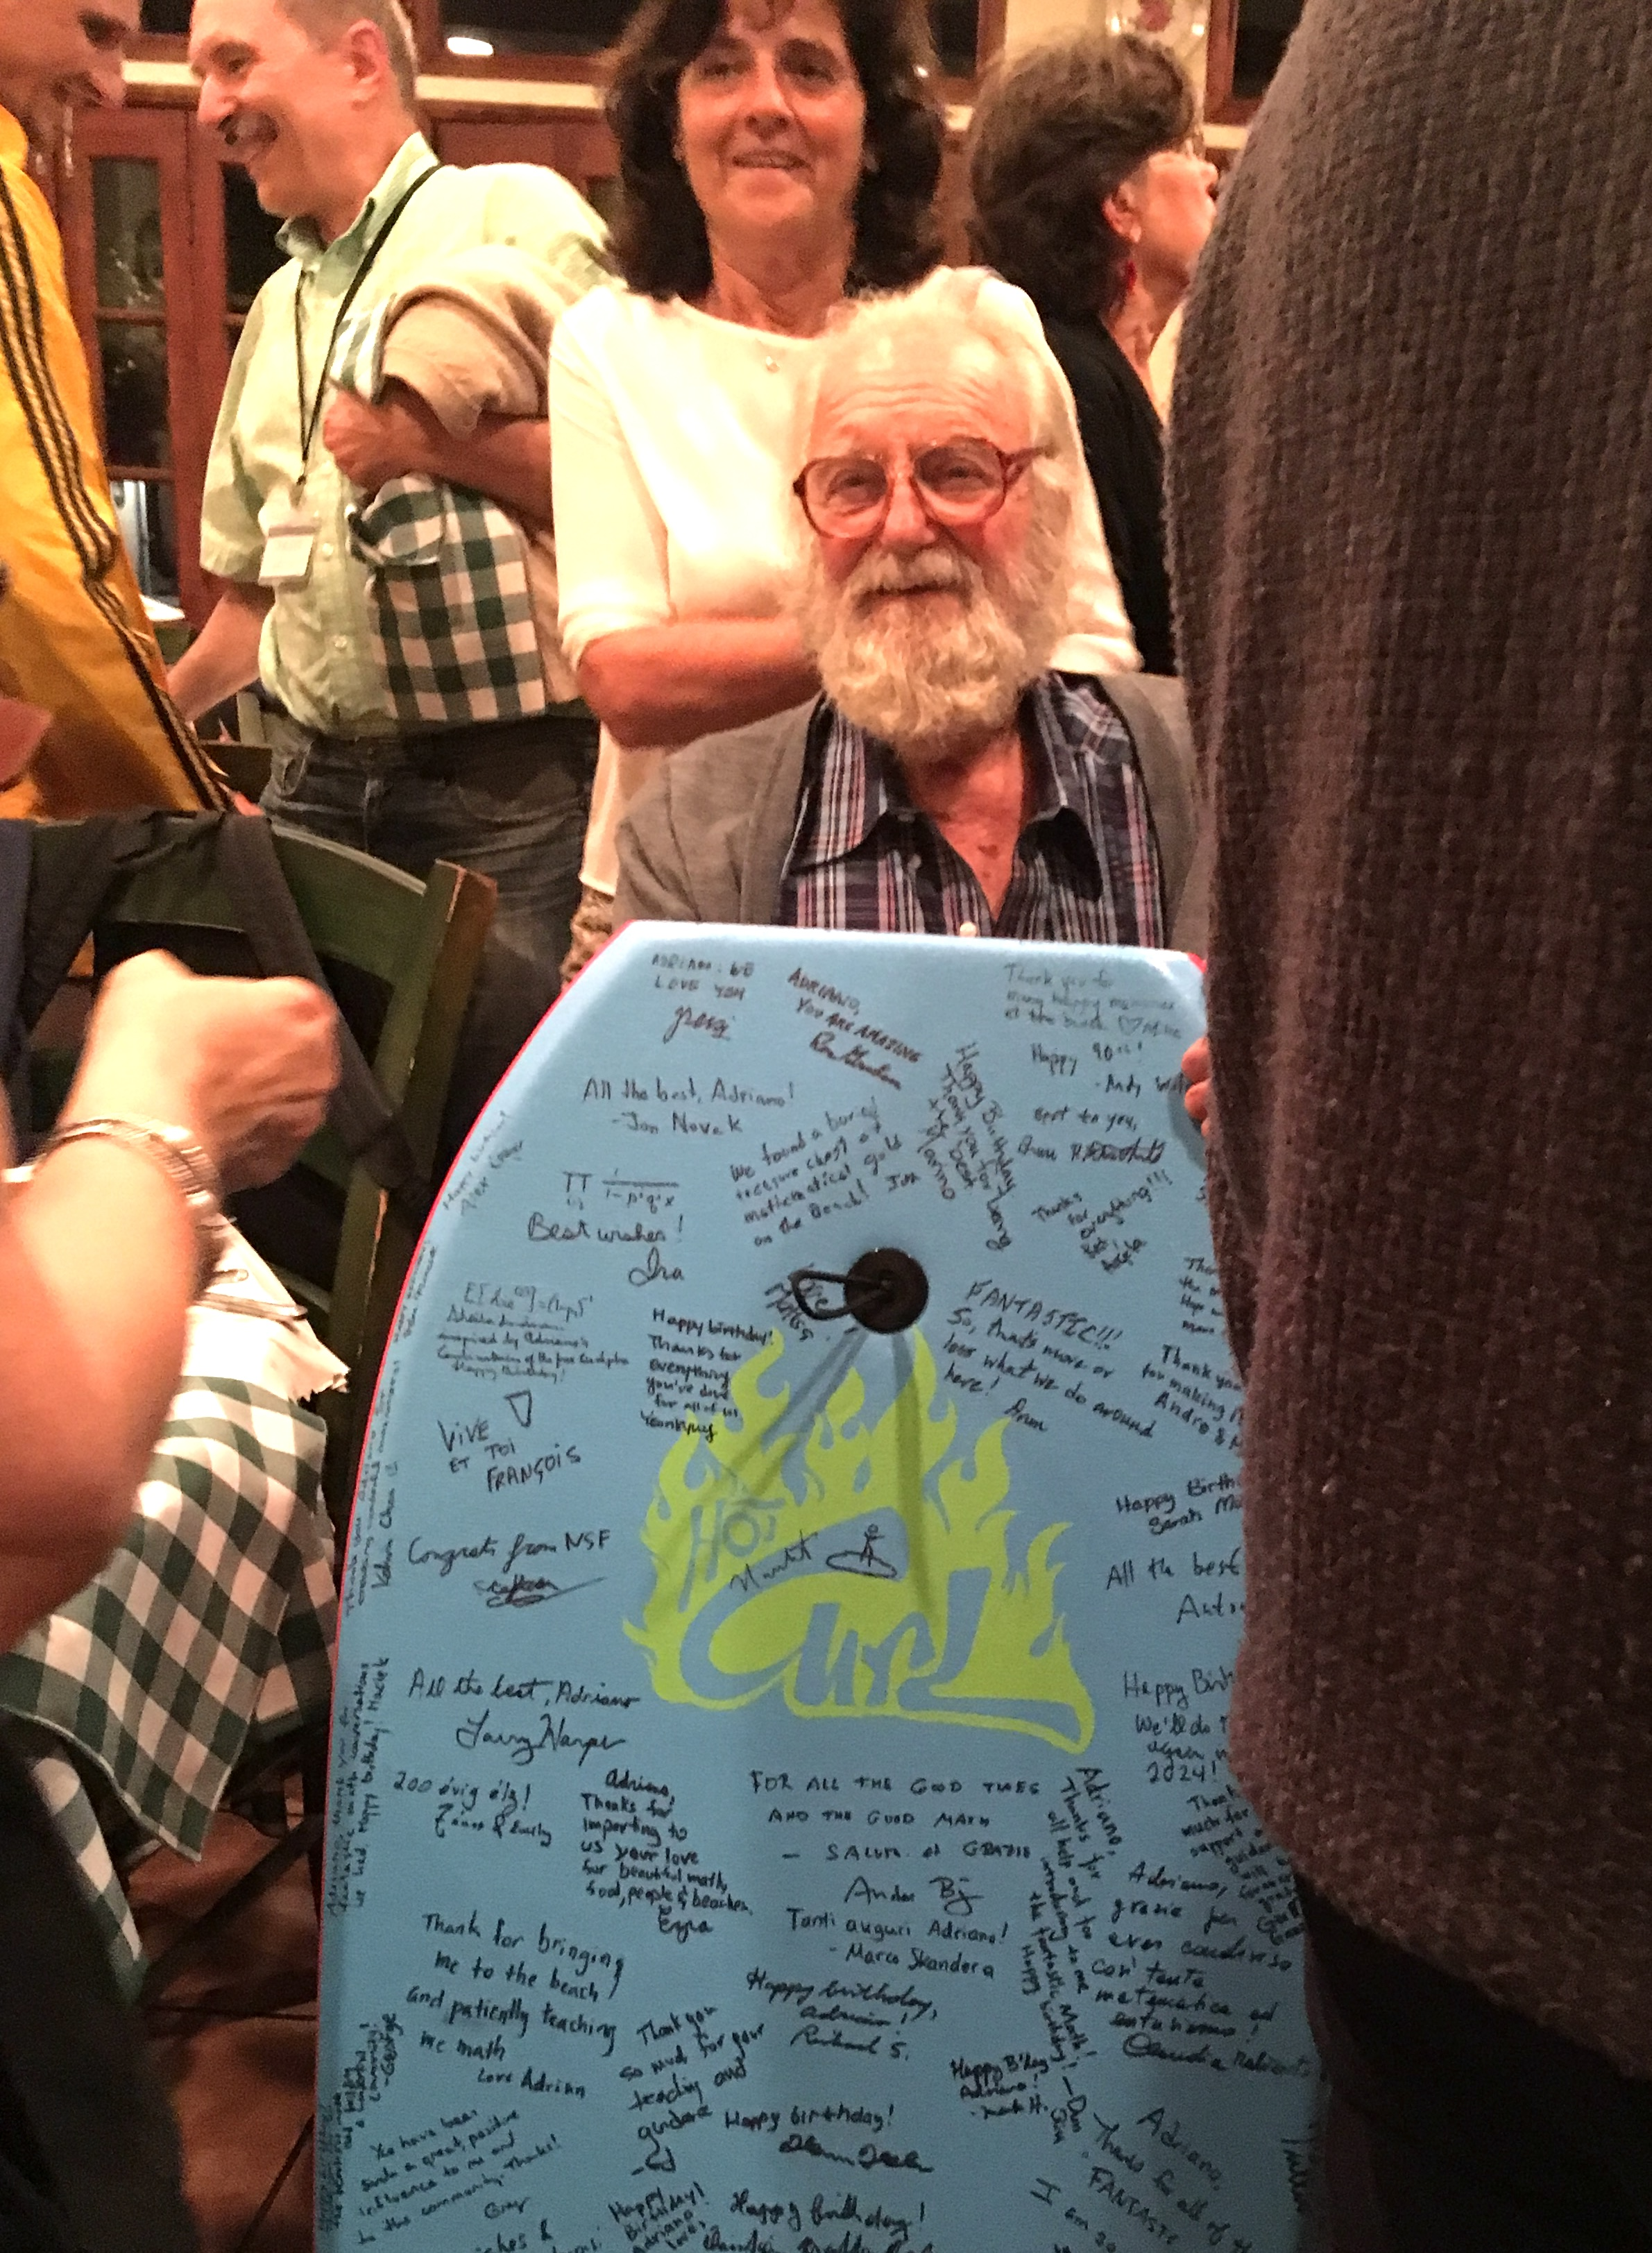
\includegraphics[width=0.95\linewidth]{Michelle_Wachs/IMG_4082.jpeg} 
 {\footnotesize Adriano, Diane, and the Boogie Board at Garsiafest, Scripps, 2019}
    \end{wrapfigure}
The beach was Adriano's second office. 
His students, collaborators, and many distinguished visitors would find him at his  encampment on the beach (first in Del Mar, later at La Jolla Shores) where he would share his beautiful mathematical ideas and listen to theirs. He also shared his passion for riding the waves.    He got a Morey Boogie Board when they first came out in 1975, and after seeing his, I went right to the store to get one too. In the years to come he would bring a stack of them to the beach for his visitors to use.  At his 91st birthday conference -- held appropriately at the Scripps Institute of Oceanography overlooking the beach -- a boogie board signed by all the participants was presented to him.  The NSF program director remarked in his speech at the conference that  Adriano, at $91$, was the oldest active principal investigator on an NSF grant in any scientific field. 

\begin{wrapfigure}{r}{0.35\textwidth}
    \centering
    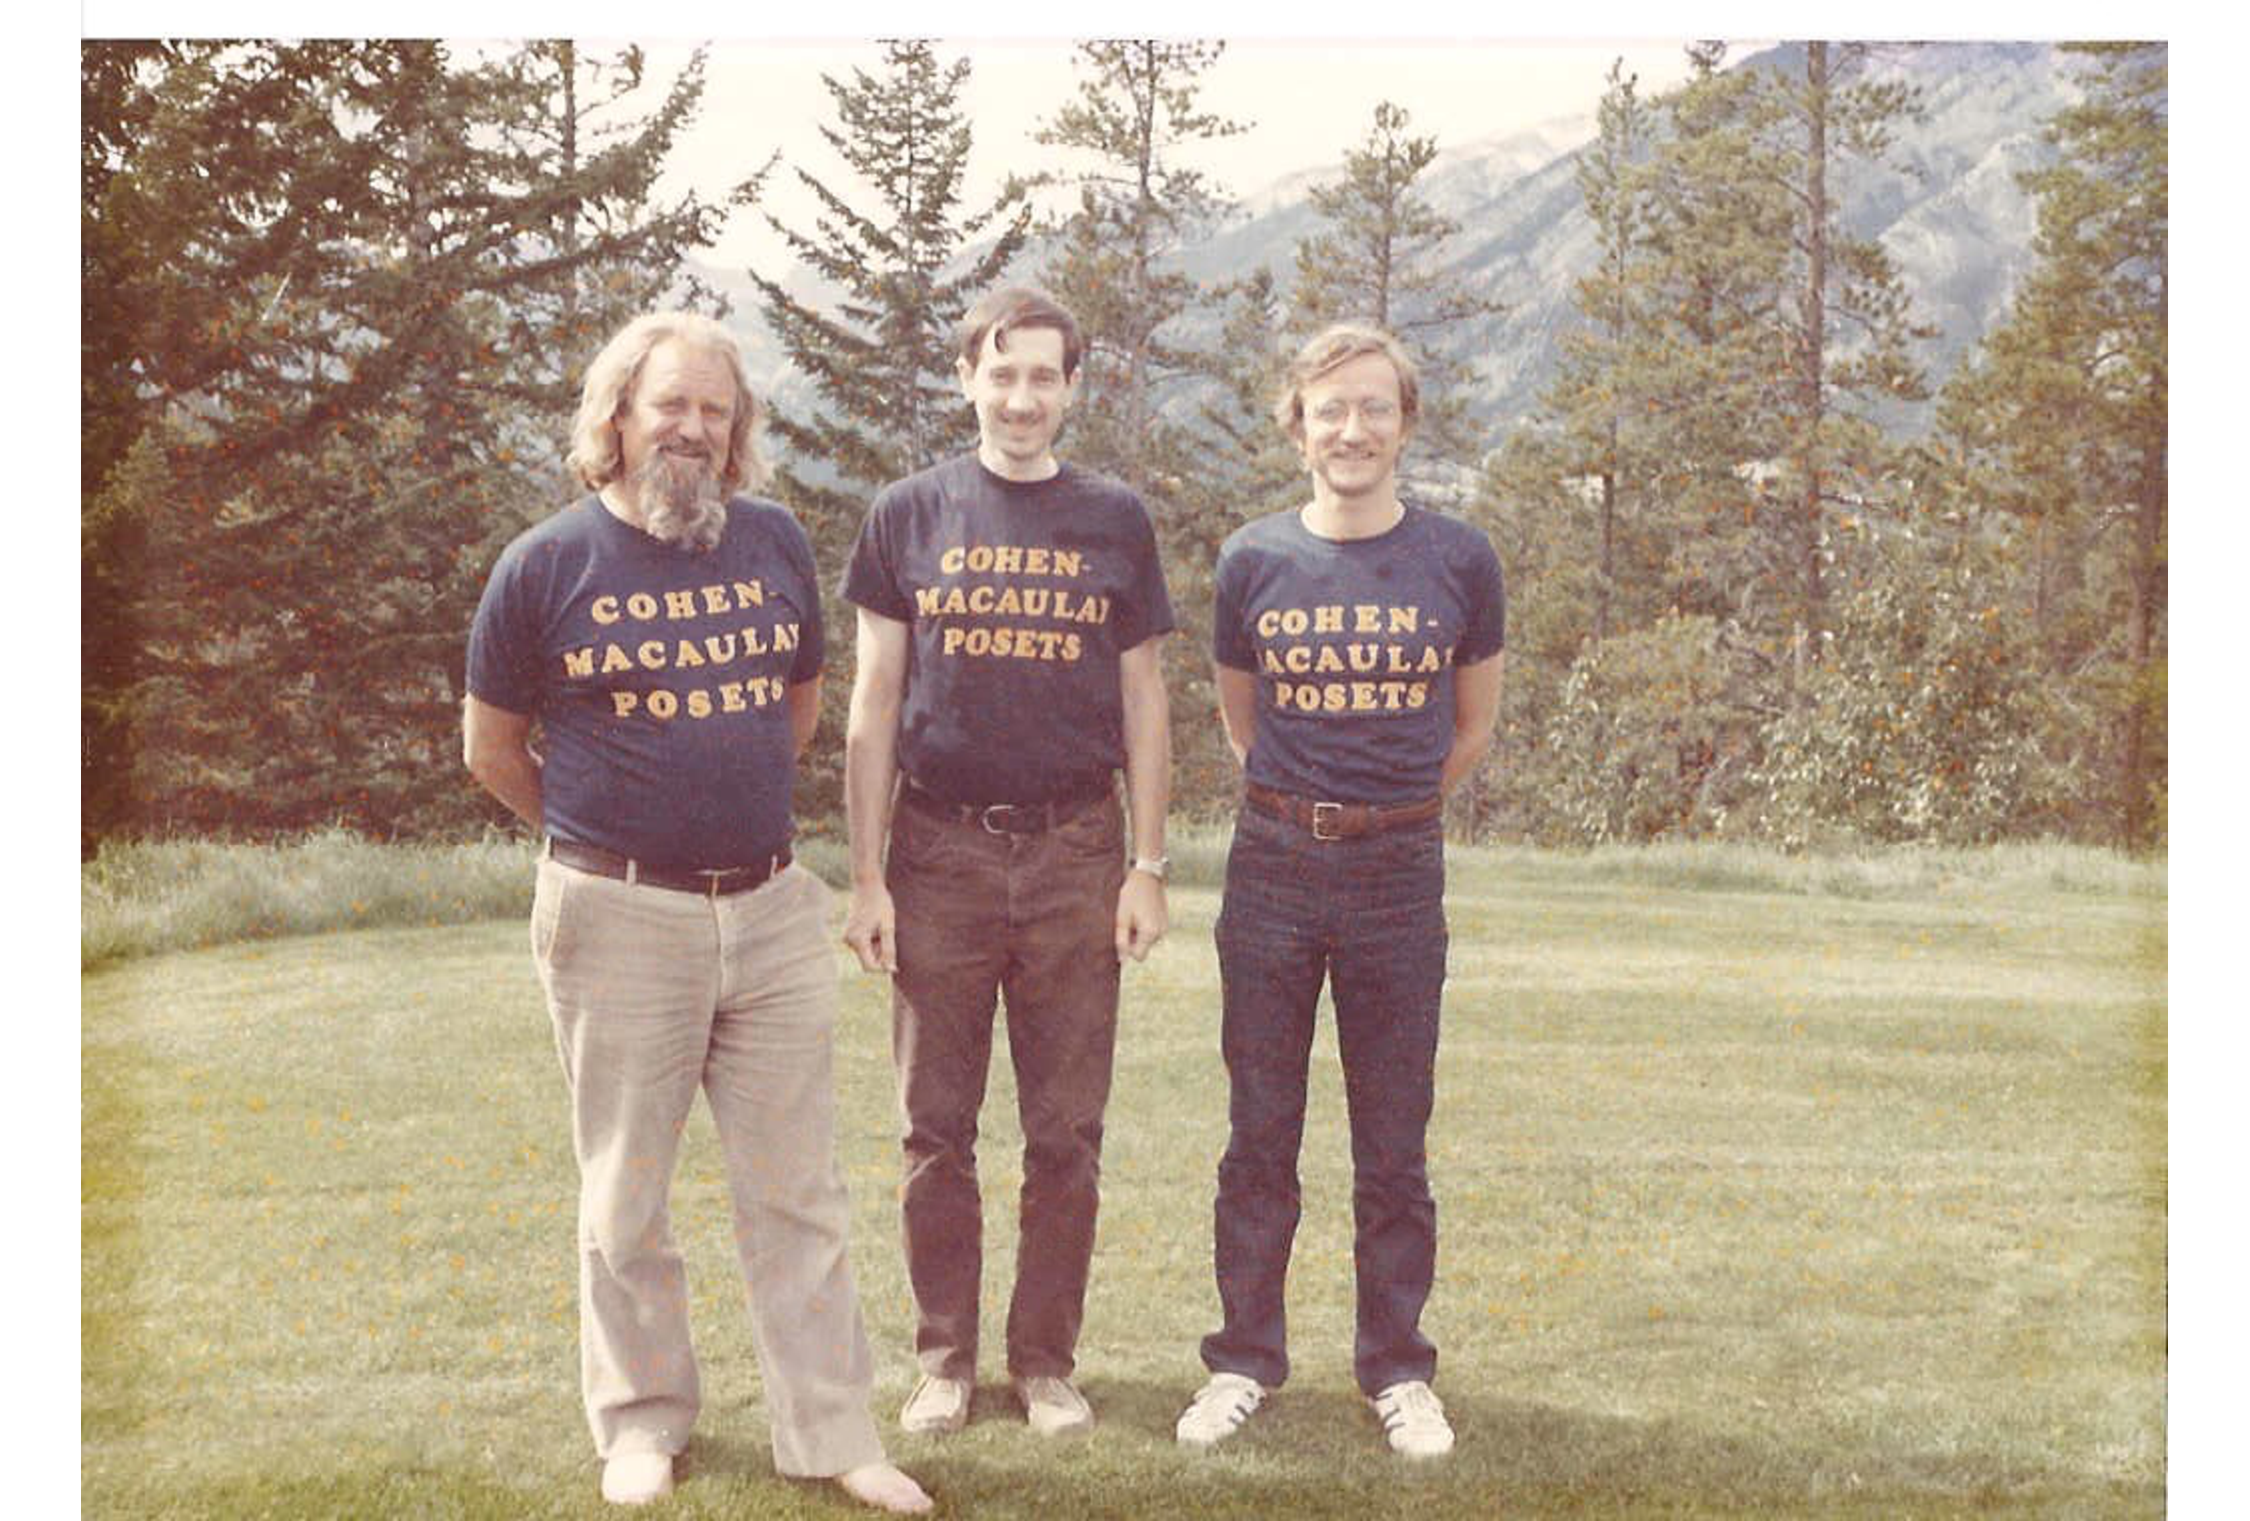
\includegraphics[width=0.95\linewidth]{Michelle_Wachs/cmposets.pdf} 
  {\footnotesize Adriano, Richard, Anders at Banff Conference on Ordered Sets, 1981}
    \end{wrapfigure}
From the mid-1970s to the late-1980s, Adriano's pioneering work helped shape the field of algebraic combinatorics and made him  one of the field's true founding leaders. So many of the ideas he introduced during that  period continue to influence the field today. I’d like to share just a few threads from that time that have had a deep and lasting impact on my own work.
 Adriano’s early research on 
q-analogs and symmetric functions -- much of it done in collaboration with Ira Gessel and Jeff Remmel -- laid the groundwork for his later celebrated work with Mark Haiman on Macdonald polynomials and diagonal harmonics. Those early papers -- as well as his subsequent papers --  were also a key source of inspiration for my own research on 
q-analogs and symmetric functions throughout my career. His work on Cohen-Macaulay posets, including his influential survey chapter  with Anders Bj\"orner and Richard Stanley, played a central role in the early development of topological combinatorics,  a field I’ve been fortunate to be part of since  early in my career. And Adriano’s beautiful work on the Lie representation of the symmetric group continues to resonate with me. It sparked ideas that led to some of my own early research and has remained a source of insight and motivation in my work on this topic ever since.

Adriano was an exceptional advisor -- extremely generous with his time and ideas. He had a rare gift for recognizing and nurturing the individual talents and abilities of his students.   Many of us feel we owe what ever success we have achieved to his mentorship.  In addition to sharing his great ideas, he was supportive and passionate.  His excitement about our work was a great confidence booster.  He and I often had spirited debates when discussing math,  but we always resolved things amicably.   The good thing was that I always felt free to express myself openly and honestly. 

Adriano was there for his students long after they graduated.    For many years after completing my Ph.D., my husband (a fellow UCSD Ph.D. -- in differential geometry)  and I would spend the summers visiting UCSD, and we even spent a full academic year there as visiting associate professors.   
Adriano helped make this possible by being a wonderful mathematical host and finding  places for us to stay.   
During those visits, there was a vibrant atmosphere in algebraic combinatorics, with seminars given
\begin{wrapfigure}{r}{0.3\textwidth}
 \centering
    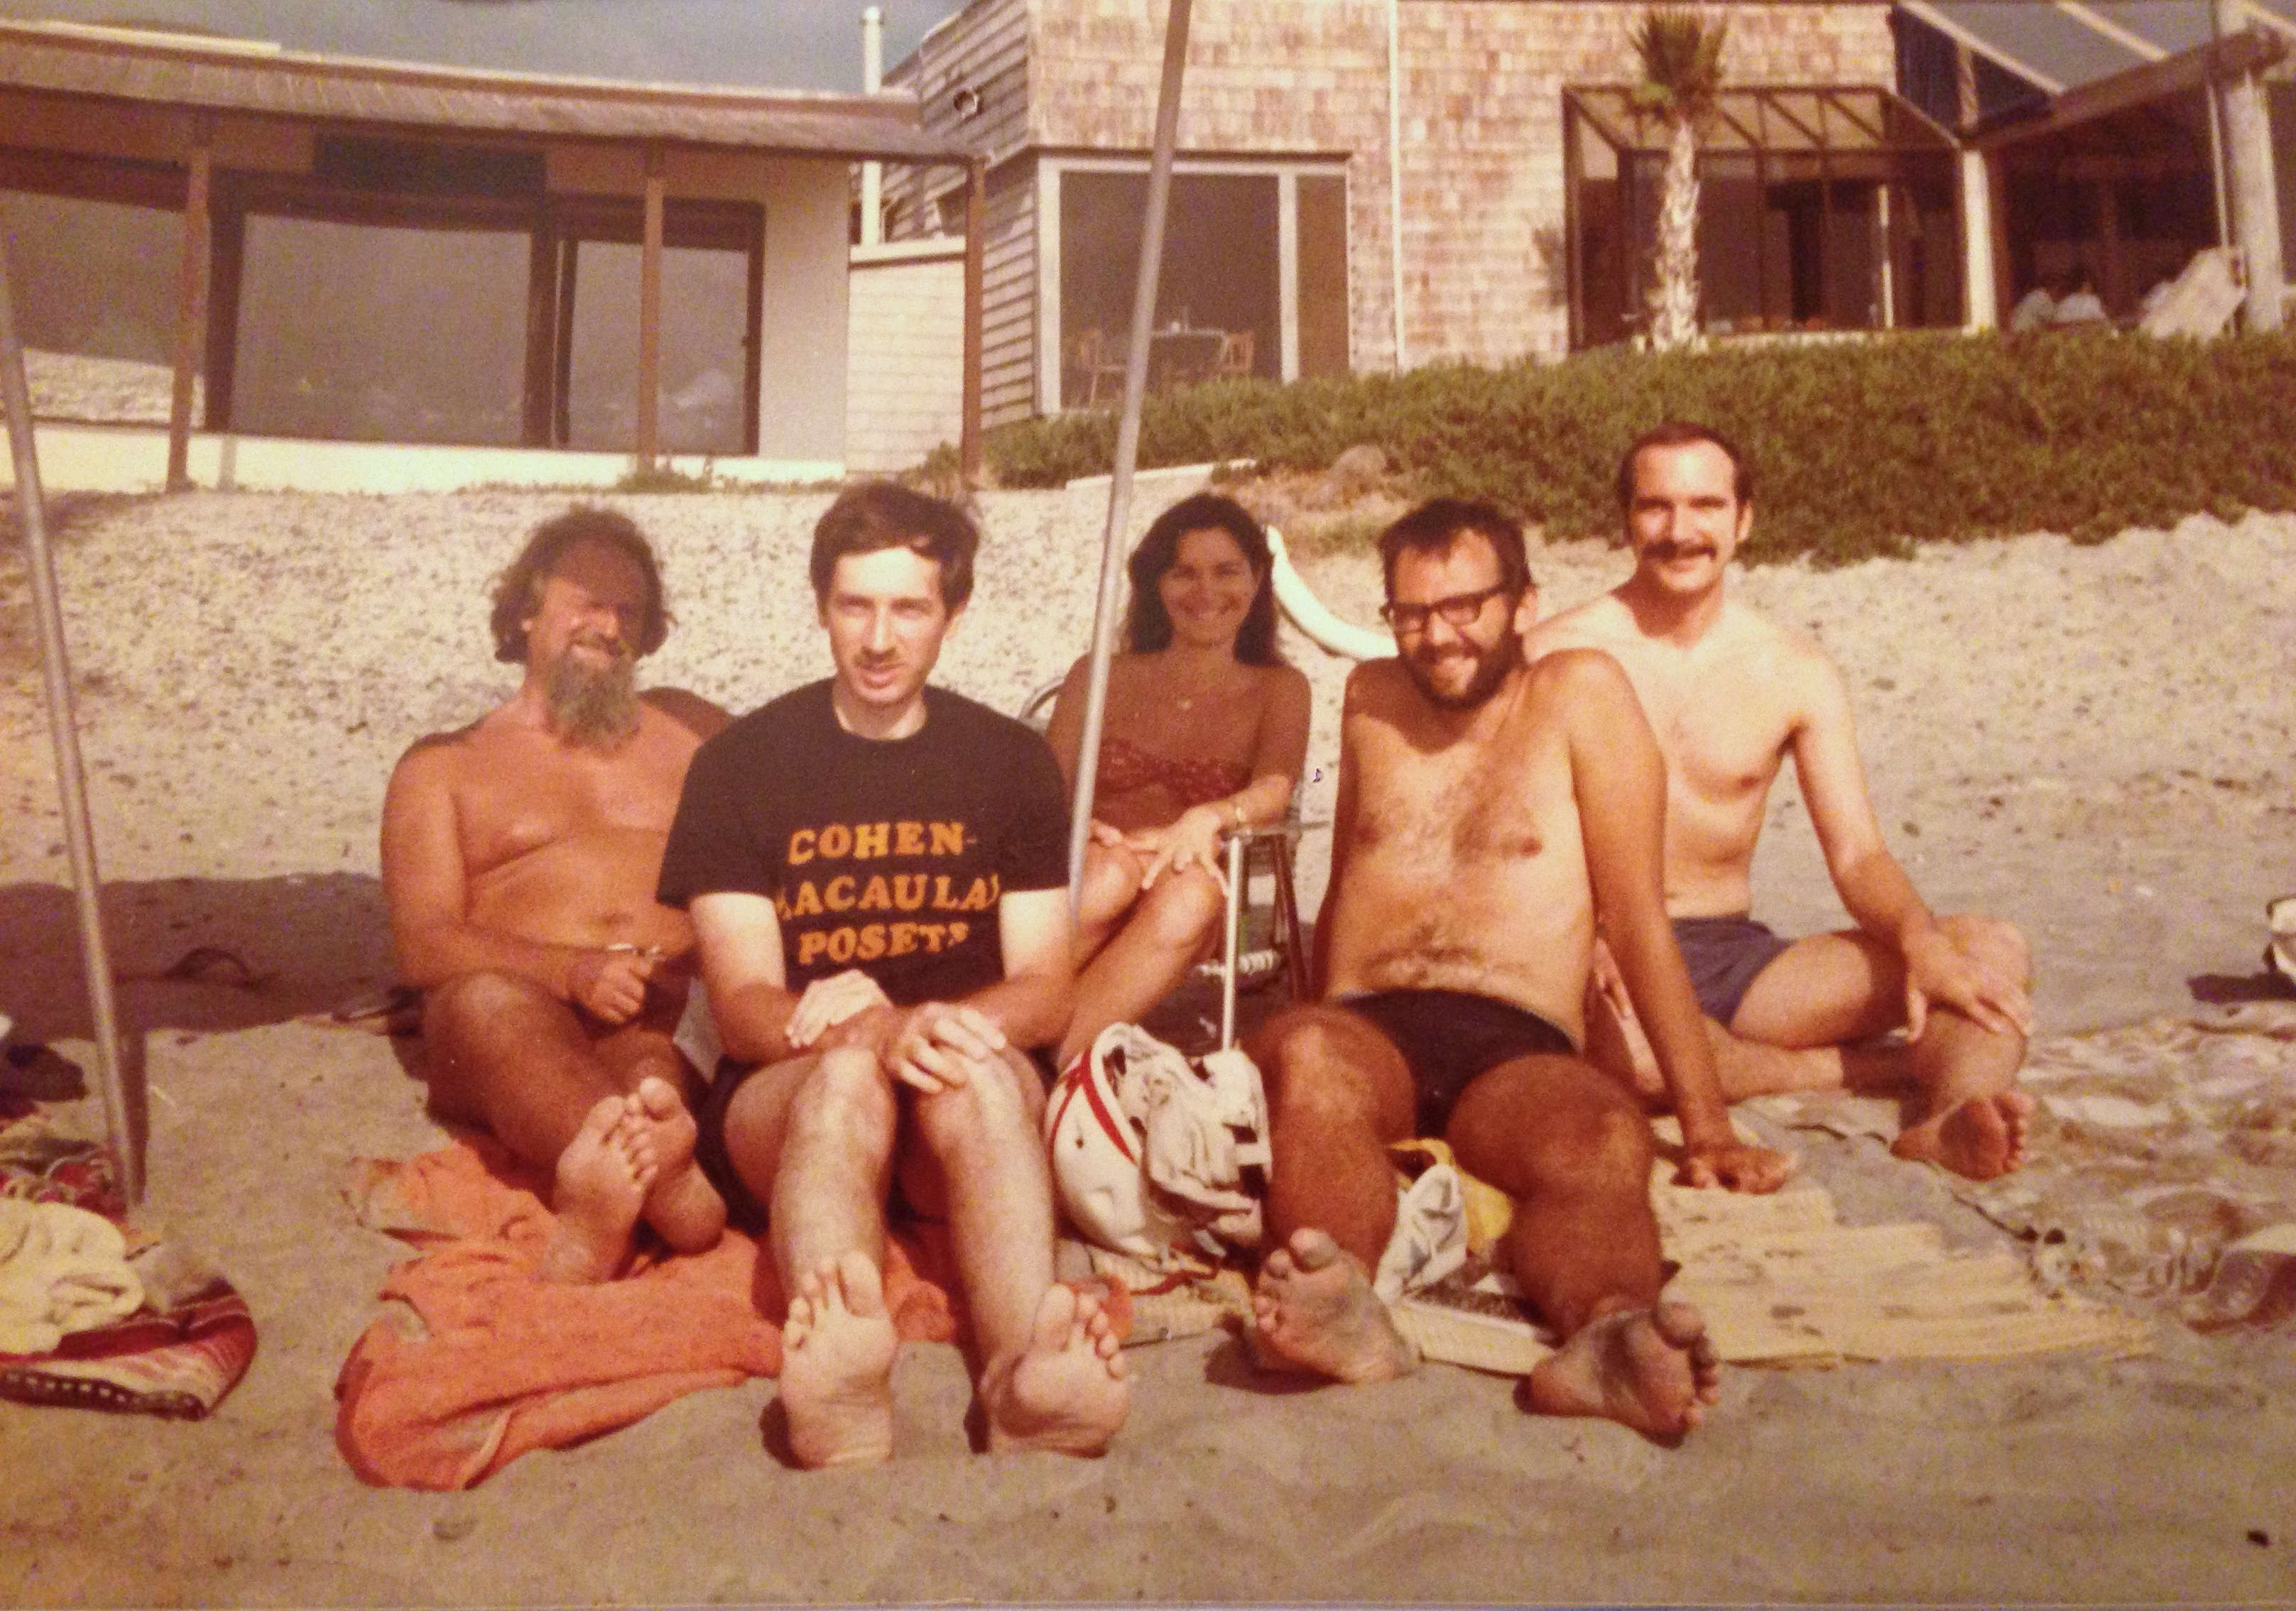
\includegraphics[width=0.95\linewidth]{Michelle_Wachs/IMG_2458.jpg} 
  {\footnotesize UCSD Combinatorics Seminar, Del Mar, 1981, Adriano, Richard, me, Dennis, Jeff}
\end{wrapfigure}
by distinguished visitors such as Richard Stanley, Anders Bj\"orner, Alain Lascoux, and Dennis Stanton, to name a few. 
 During my first summer visit, Adriano suggested to Anders that he discuss with me his problem  on shellability of Bruhat order.   This led to a lifelong collaboration and friendship with Anders for which I remain deeply grateful to Adriano. This was typical Adriano-he fostered many enduring mathematical relationships.

My husband Greg and I took some memorable trips with Adriano and his wife Diane, both mathematical and personal.  We had a great time in Rome with Adriano teaching us all how to behave in Italy and how to sniff out good restaurants. Our young children, Brian and Gabriela, were inseparable during our stays in 1992 at Mittag-Leffler and in 1994 at Garsiafest in Taormina. Whether at home or away,  Adriano loved to entertain his colleagues and friends by treating us to unforgettable Italian and Tunisian meals, which he cooked himself.

\begin{center}
 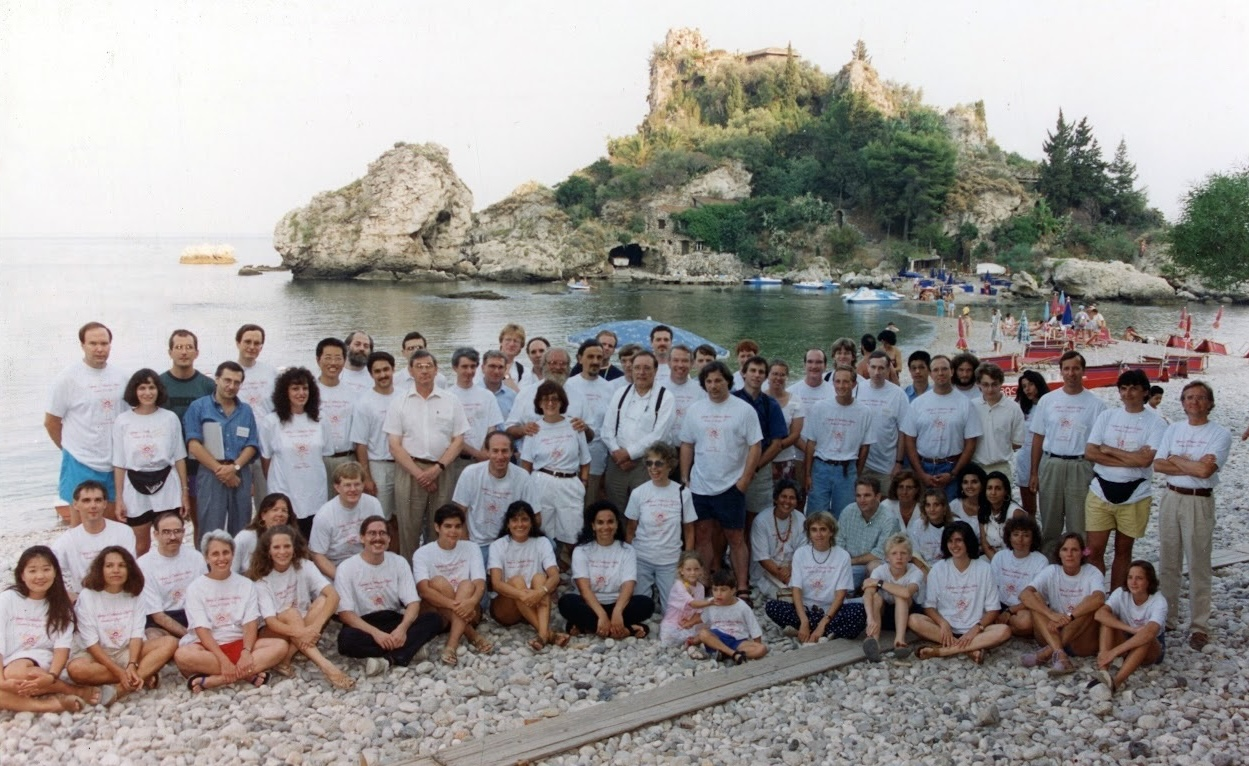
\includegraphics[height=1.7in]{Michelle_Wachs/EmbeddedImage.jpeg} 
 \\ {\footnotesize Garsiafest, Taormina, 1994}
\end{center}

To so many of us, Adriano was more than a mentor, colleague, or friend--he was family.  Once, during a short visit to San Diego, he and Diane invited me to stay with them. At the time, their two-bedroom country home  was full, with Diane’s brother occupying the second room.  So my ``room'' was the front porch.   I left my suitcase in the living room while I slept out on the porch.  My suitcase was a  beat-up leather suitcase with a handle that had become partially detached.  When I came in the next morning, to my surprise, Adriano  was busy sewing the handle back on with a giant needle and thick thread. I was so touched. What could be sweeter and more fatherly than that?  

Adriano’s passion for mathematics--and for life--was legendary.  His work continues to have a strong influence on my work and that of so many others.  What a profound privilege it has been to have known this remarkable man for so many years.

\section*{Nantel Bergeron}
Of course, when thinking about Adriano, countless dinner stories come to mind. He was passionate about life, and it was around the making and enjoyment of food that one got to know him more deeply. From stories of his childhood to tales about mathematics, Adriano was an open book filled with fascinating plots and anecdotes.

I always felt that Adriano was part of my family--and that I was part of his. 

\begin{figure}[h]
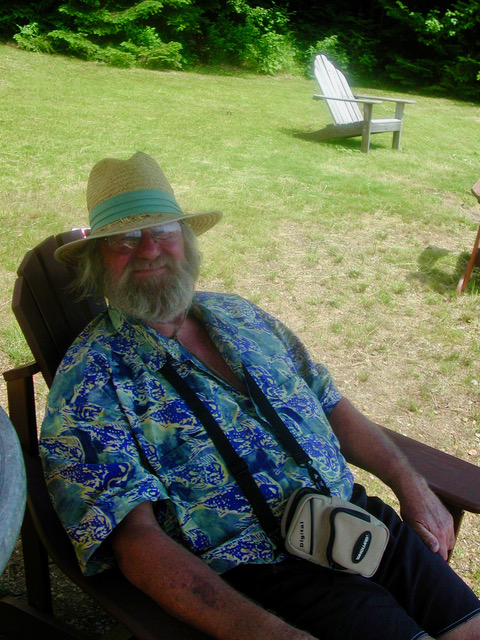
\includegraphics[width=2.5in]{Nantel_Bergeron/DSCN3064.jpeg}

{\footnotesize Adriano at my cottage near Mont Tremblant, Quebec. We would often gather where there is water.}
\end{figure}

Slowly, through these wonderful dinners, I was introduced to some of the most influential mathematicians of the time! I still remember the day Schützenberger visited UCSD and Adriano wanted to cook dinner for the master. At the time, he was in transition between houses, so he used my apartment to cook. I was incredibly intimidated to host Schützenberger--this was quite something for me. And I must say, it was the first time I felt that Adriano himself was also a little bit intimidated. Perhaps he even expressed it more than he felt, just to make me feel at ease. I wouldn’t be surprised--this would be so in line with his nature.

Yes, this was a wonderful life! But somehow, mathematics was always there--woven into everything. It is through mathematics that I discovered a very different mind. I remember him going through pages of computations. Sometimes I would follow line by line, only realizing at the end the scope of what we had done. I would always marvel at that moment--``How did he do it?'' And again, he would make me feel comfortable, point to something I had done that he found wonderful.

I saw him get so excited about what those around him had accomplished, especially us--his students. In fact, that’s how he recruited me to study in San Diego in 1987. We had worked on some small representation theory problems in Montreal, and since I had solved a minor question, he got all excited and convinced me to give up my plans to go into physics and instead study with him at UCSD.

I am sure many of his students will recognize themselves in these stories.

Thank You Adriano

\end{document}
